\documentclass[12pt,twoside]{article}
\usepackage{amsmath, amssymb}
\usepackage{amsmath}
\usepackage{fancyhdr,parskip}
\usepackage[active]{srcltx}
\usepackage{amssymb}
\usepackage{amscd}
\usepackage{makeidx}
\usepackage{amsthm}
\usepackage{algorithm}
\usepackage{algpseudocode}
\usepackage{fancyhdr}
\usepackage{graphics}
\usepackage{amsmath, amssymb}
\usepackage{amsmath}
\usepackage[active]{srcltx}
\usepackage{amssymb}
\usepackage{amscd}
\usepackage{makeidx}
\usepackage[dvips]{graphicx}
\usepackage{longtable}
\usepackage{tabularx}
\usepackage[table,xcdraw]{xcolor}
\usepackage{color}
\usepackage[hidelinks]{hyperref}
\usepackage[backend=biber,style=apa]{biblatex}
\usepackage{longtable}
\usepackage{tabularx}
\usepackage[table,xcdraw]{xcolor}
\usepackage{color}
\usepackage[hidelinks]{hyperref}
\usepackage{multirow}
\usepackage{algorithm}
\usepackage{algpseudocode}
\renewcommand{\algorithmicrequire}{\textbf{Input:}}
\renewcommand{\algorithmicensure}{\textbf{Output:}}
\renewcommand{\tablename}{Tabla}
\renewcommand{\figurename}{Figura}
\renewcommand{\baselinestretch}{1}
\setcounter{page}{1}
\setlength{\textheight}{21.6cm}
\setlength{\textwidth}{14cm}
\setlength{\oddsidemargin}{1cm}
\setlength{\evensidemargin}{1cm}
\pagestyle{myheadings}
\thispagestyle{empty}
\markboth{\small{Pr\'actica 3. Luis Francisco Renteria Cedillo, Denzel Omar Vazquez Perez.}}{\small{.}}
\date{}
\begin{document}
    \begin{figure}[h]
    \vspace{-3cm} \hspace{-2cm} \setlength{\unitlength}{1mm}
    \begin{picture}(15,25)(-10,0)
    
\includegraphics[width=16.5cm,height=2.8cm]{imagenes/titulo.png}
    \end{picture}
    \end{figure}
    \vspace{0cm}
    \centerline{\bf An\'alisis de Algoritmos, Sem: 2022-2, 3CV11, Pr\'actica 3, 03 de abril de 2022}
    \centerline{}
    \begin{center}
    \Large{\textsc{Pr\'actica 3: Funciones Recursivas vs Iterativas}}
    \end{center}
    \centerline{}
    \centerline{\bf {Luis Francisco Renteria Cedillo, Denzel Omar Vazquez Perez.}}
    \centerline{}
    \centerline{$lrenteriac1400@alumno.ipn.mx, dvazquezp1600@alumno.ipn.mx$}
    \newtheorem{Theorem}{\quad Theorem}[section]
    \newtheorem{Definition}[Theorem]{\quad Definition}
    \newtheorem{Corollary}[Theorem]{\quad Corollary}
    \newtheorem{Lemma}[Theorem]{\quad Lemma}
    \newtheorem{Example}[Theorem]{\quad Example}
    \bigskip
    \textbf{Resumen:} Se realiza el análisis y comparaciones entre algoritmos recursivos e iterativos, con el objetivo de determinar el grado de complejidad para cada uno de ellos. Se llevaron a cabo análisis a priori y posteriori, para determinar el orden de complejidad de manera teórica y práctica.

    {\bf Palabras Clave:}Lenguaje C, Análisis, Recursividad, Iterativo, Algoritmos
    
    \section{Introducci\'on}
    
     
    
    Dentro de los lenguajes de programación, las estructuras de control permiten establecer un flujo de datos según las instrucciones de un programa.Un ciclo o bucle es ampliamente usado para definir un conjunto de instrucciones que se ejecutaran n numero de veces hasta que una condición de control lo permita.
    
    Con la llegada de problemas más complejos y extensos, llegó la programación modular, que utiliza la técnica de "Divide y Vencerás", donde su principal objetivo es dividir el problema en pequeños módulos para facilitar su posterior solución individual. Dichos módulos, en la práctica, se les conoce comúnmente como funciones, métodos o procedimientos.
    
    Un algoritmo puede implementarse en un lenguaje de programación como una función, donde esta debe de definirse con un nombre, un tipo de dato a regresar, un conjunto de parámetros o argumentos y un conjunto de instrucciones a ejecutar. Es aquí cuando técnicas como recursividad o iteración son utilizados para resolver diversos problemas, mismos que serán explicados en la siguiente sección.
    
    
    
    \section{Conceptos te\'oricos}
    
    
        \subsection{Algoritmos Recursivos}
        Un algoritmo recursivo utiliza la técnica de "divide y vencerás", donde el problema principal se divide en varios subproblemas que tienen características muy similares.
        
        La recursividad está estrechamente relacionado con funciones recurrentes e incluso fractales, ya que la recursividad implica construir o generar, a partir de características de si mismo o mismo tipo.
        
        En ciencias de la computación, la recursividad es un proceso en donde uno de sus pasos es invocar al mismo proceso. Esta técnica es un pilar fundamental para otras técnicas como lo es la programación dinámica.
        
        \subsection{Algoritmos Iterativos}
        Un algoritmo iterativo es aquel que se ejecuta dentro de un ciclo mientras que un conjunto de condiciones lo permitan. A comparación de un algoritmo recursivo, un algoritmo iterativo es generalmente más extenso en su escritura.
        
    \subsection{Pseudocódigos de los problemas a analizar}
    Nuestro primer problema a analizar serán tres algoritmos diferentes que calculan el cociente de una división de números enteros. Cada función tiene una forma diferente de llegar al mismo resultado, ya sea usando funciones recursivas o iterativas.
    
    A continuación se mostrarán los pseudocódigos de dichas funciones:
    
    \begin{algorithm}[H]
        \caption{Division1}
        \begin{algorithmic}[1]
        \Require{$int~n,~int~div,~int~res$} 
        \Ensure{cociente(n/div)}
        \State q = 0
        \While{$n\geq div$}
            \State n = n-div
            \State q = q+1
        \EndWhile
        \State res = n
        \State return q
        \end{algorithmic}
    \end{algorithm}
    \begin{algorithm}[H]
        \caption{Division2}
        \begin{algorithmic}[1]
        \Require{$int~n,~int~div,~int~res$} 
        \Ensure{cociente(n/div)}
        \State dd = div
        \State q = 0
        \State r = n
        \While{$dd\leq n$}
            \State dd = (2)(dd)
        \EndWhile
        \While{$dd>div$}
            \State dd = dd/2
            \State q = (2)(q)
            \If{$dd\leq r$}
                \State r = r - dd
                \State q = q + 1
            \EndIf
        \EndWhile
        \State return q
        \end{algorithmic}
    \end{algorithm}
    \begin{algorithm}[H]
        \caption{Division3}
        \begin{algorithmic}[1]
        \Require{$int~n,~int~div,~int~res$} 
        \Ensure{cociente(n/div)}
        \If{$div~>~n$}
            \State return 0
        \Else
            \State return 1+Division3(n-div,div)
        \EndIf
        \end{algorithmic}
    \end{algorithm}
    
    La segunda parte del problema a analizar serán dos algoritmos de búsqueda, uno recursivo y otro iterativo, que tienen como objetivo encontrar un numero $K$ en un arreglo, esto al dividir este en tres partes iguales y comparar con los extremos interiores $i$ y $j$. 
    
    A continuación se mostrarán los pseudocódigos de dichas funciones:
    
    \begin{algorithm}[H]
        \caption{search\_num}
        \begin{algorithmic}[1]
        \Require{$int~A[],~int~n,~int~inicio,~int~final$} 
        \Ensure{N\'umero natural}
        \While{inicio$\leq$final}
        \State i = inicio + ((final-inicio)/3)
        \State j = inicio + (2*((final-inicio)/3))+1
        \If{n==A[i]}
        \State return i
        \ElsIf{n==A[j]}
        \State return j
        \ElsIf{n$<$A[i]}
        \State final = i-1
        \ElsIf{n$>$A[j]}
        \State inicio = j+1
        \Else
        \State final = j-1;
        \State inicio = i+1;
        \EndIf
    	\EndWhile
    	\State return -1
        \end{algorithmic}
    \end{algorithm}
    \begin{algorithm}[H]
        \caption{search\_num\_R}
        \begin{algorithmic}[1]
        \Require{$int~A[],~int~n,~int~inicio,~int~final$} 
        \Ensure{N\'umero natural}
        \State i = inicio + ((final-inicio)/3)
        \State j = inicio + (2*((final-inicio)/3))+1
        \If{inicio$>$final}
            \State return -1
        \EndIf
        \If{n==A[i]}
            \State return i
        \ElsIf{n==A[j]}
            \State return j
        \ElsIf{n$<$A[i]}
            \State search\_num\_R(A, n, inicio, i-1)
        \ElsIf{n$>$A[j]}
            \State search\_num\_R(A, n, j+1, final)
        \Else
            \State search\_num\_R(A, n, i+1, j-1);
        \EndIf
        \end{algorithmic}
    \end{algorithm}
    \section{Experimentaci\'on y resultados}
        \subsection{Algoritmos de la divisi\'on}
            \subsubsection{\large Divisi\'on 1}
                {\bf 3.1.1.1 An\'alisis a Priori}
                \\[0.5cm]
                En la Figura 1 podemos observar la implementación de la función división 1. Empleando las definiciones formales llegamos a concluir que las sentencias simples fuera del ciclo while tienen una complejidad de O(1), mientras que la del propio ciclo while tiene complejidad de O(n), debido a que en cada iteración, a n se le resta el valor de div y este ciclo se repite hasta que n sea mayor a div.
                
                \begin{figure}[H]
                    \centering
                    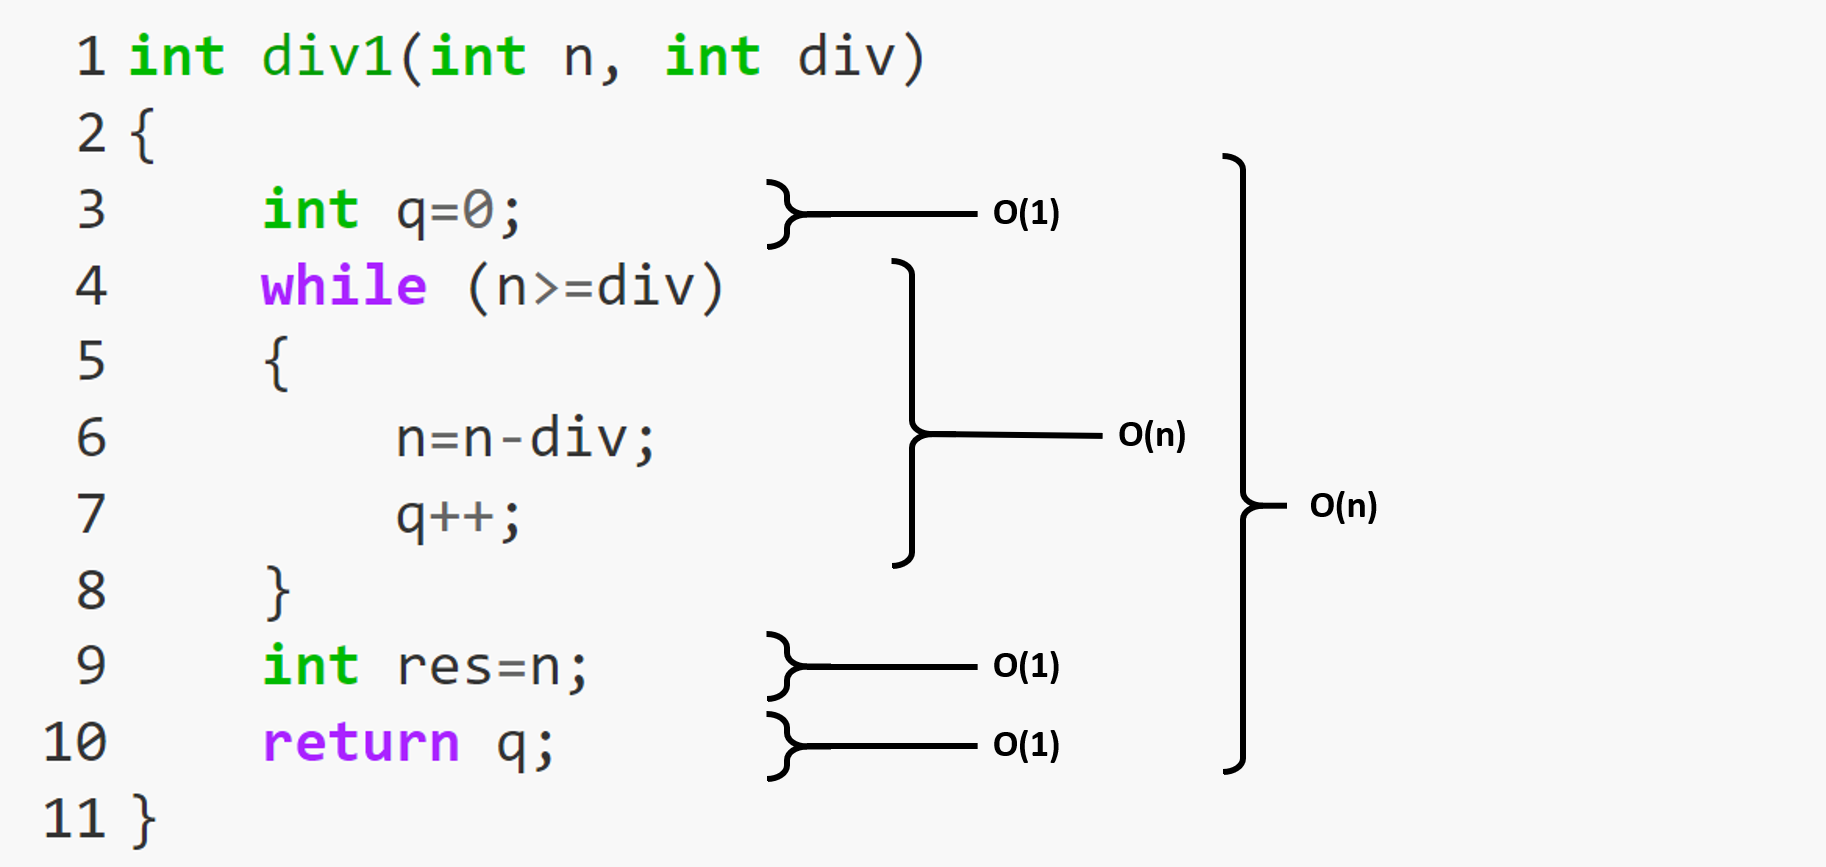
\includegraphics[width=10cm]{imagenes/divc1.png}
                    \caption{Análisis por bloques de código de la función div1().}
                \end{figure}
                
                
                {\bf 3.1.1.2 An\'alisis a Posteriori}
                
                En el siguiente gráfico que se muestra en la Figura 2 representa los conjuntos de pares ordenados los cuales representan el valor del cociente vs numero de ejecuciones. Dichos puntos se han obtenido al generar números aleatorios en el rango del 1 al 100 en el dominio de los números enteros.
                Dado el comportamiento de la gráfica, se verifica que es lineal, no habiendo diferencia entre el mejor y peor caso, y retomando que $\Theta$ se define como:
                $$\Theta(g(n)) = \{ f(n)~\arrowvert~\exists_{n}~C_{1},~C_{2}>0~\&~n_{0}>0~tal~que$$ $$0\leq~C_{1}g(n)~\leq~f(n)~\leq~C_{2}g(n)~\forall~n\geq~n_{0}\}$$
                
                
                Se proponen valores para $C_{1}=2$, $C_{2}=4$ y $n_{0}=10$. Dichos valores se acotan la parte superior como la inferior as\'i como el punto de cruce en el que se cumple la inecuación, por tanto se puede decir que $T(n)\in \Theta(n)$.

                
                \begin{figure}[H]
                    \centering
                    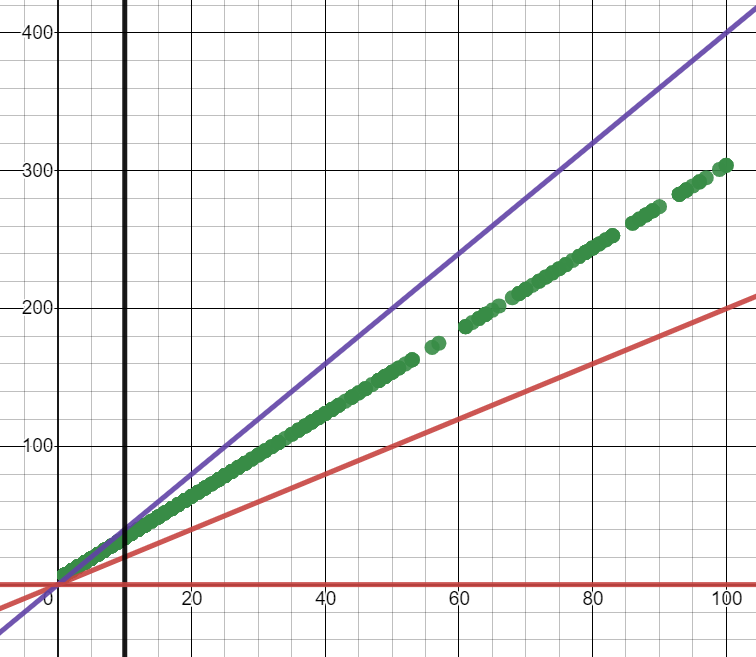
\includegraphics[width=8cm]{imagenes/div1.png}
                    \caption{Gráfico del peor y mejor caso para la función div1().}
                \end{figure}
                
                
                
            \subsubsection{\large Divisi\'on 2}
                {\bf 3.1.2.1 Analisis a Priori}
                \\[0.3cm]
                La Figura 3 muestra la implementación del código, se observa que las sentencias simples tienen complejidad O(1) mientras que las estructuras de control while tienen complejidad $O(log_2(n))$.
                
                
                
                
                \begin{figure}[H]
                    \centering
                    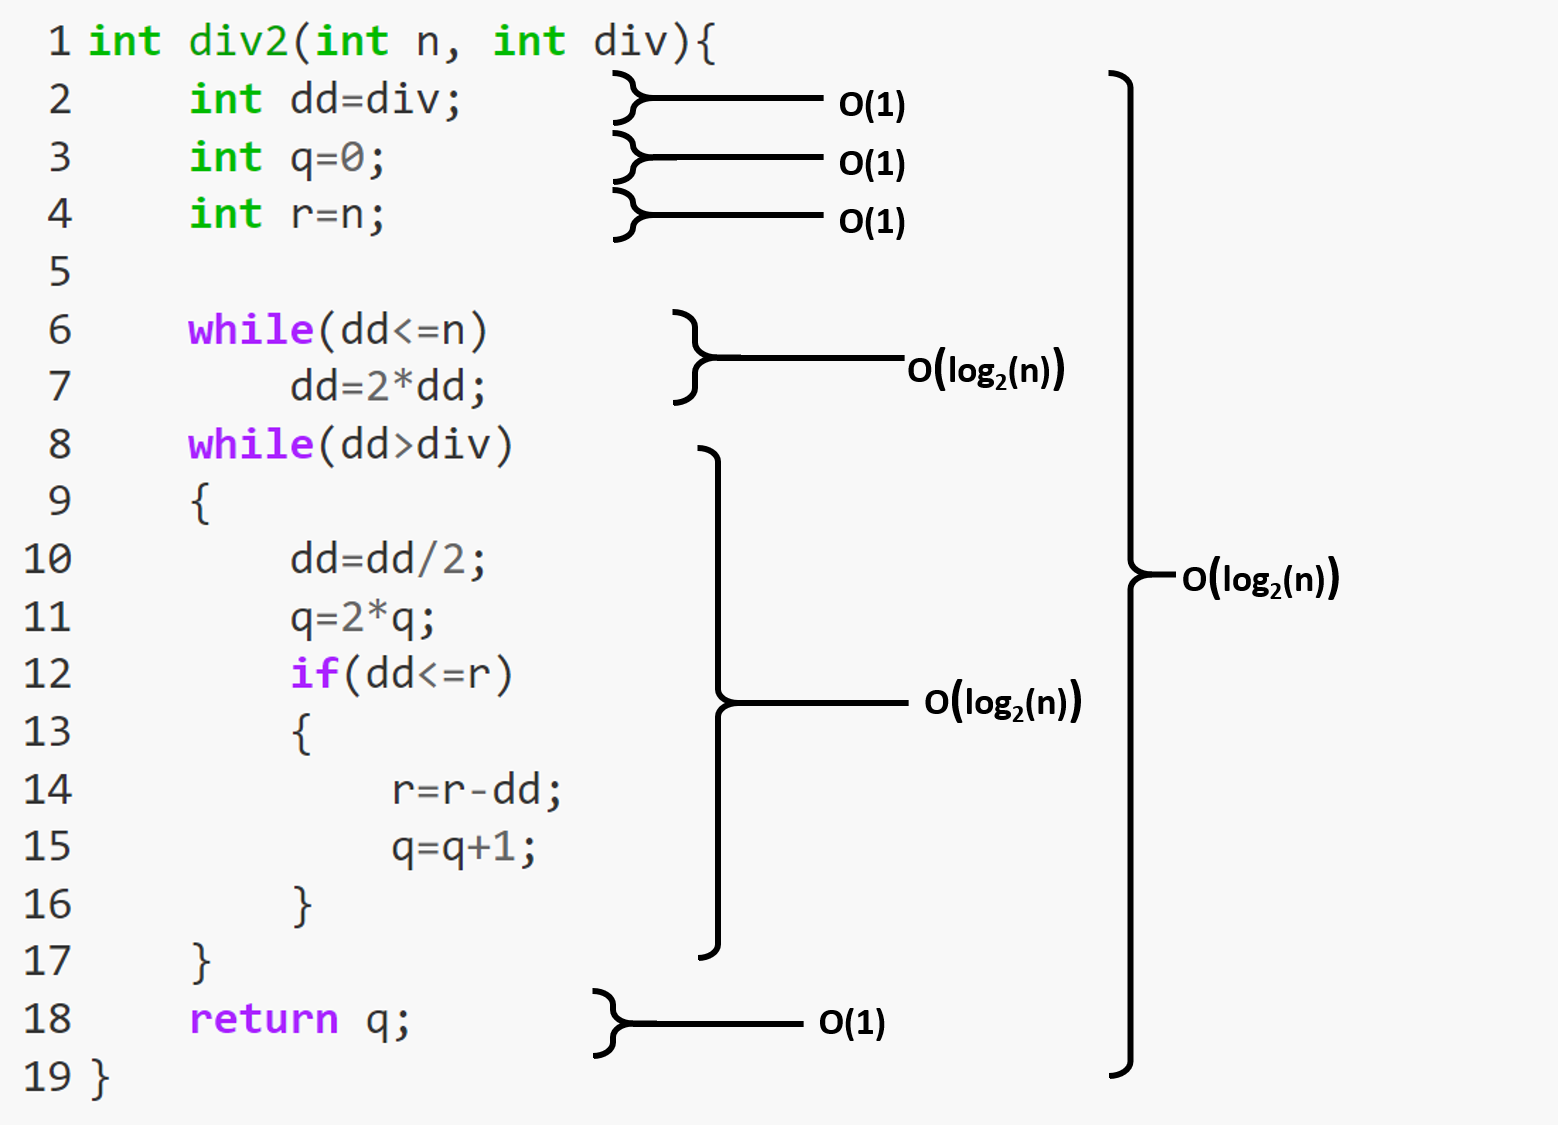
\includegraphics[width=10cm]{imagenes/divc2.png}
                    \caption{Análisis por bloques de código de la función div2().}
                \end{figure}
                
                
                {\bf 3.1.2.2 Análisis a Posteriori}
                \\[0.3cm]
                En el siguiente gr\'afico (Figura 4) se muestra el gráfico de los valores obtenidos. El comportamiento de la gráfica es logarítmico, sin diferencia entre el mejor o  el peor caso.
                Se proponen valores para $C_{1}=4$, $C_{2}=12$ y $n_{0}=10$. Dichos valores se acotan la parte superior como la inferior as\'i como el punto de cruce en el que se cumple la desigualdad, por tanto $T(n)\in \Theta (log_{2}(n))$.

                \begin{figure}[H]
                    \centering
                    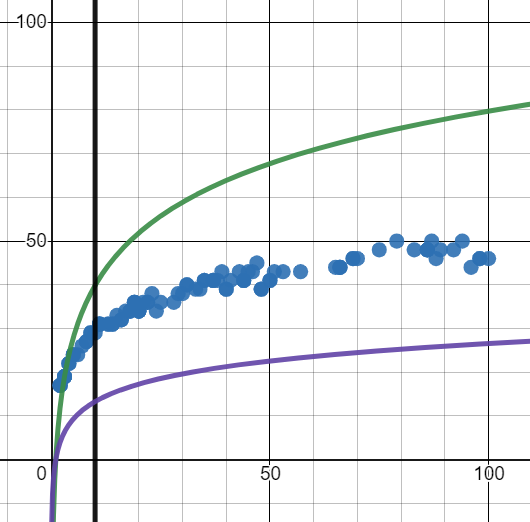
\includegraphics[width=9cm]{imagenes/div2.png}
                    \caption{Gráfico del peor y mejor caso para la función div2().}
                \end{figure}
                
                
            \subsubsection{\large Divisi\'on 3}
                {\bf 3.1.3.1 Análisis a Priori}
                \\[0.3cm]
                
                En la Figura 5 se muestra la implementación de la función división 3. Observamos que es una función recursiva que consiste en una sentencia if, la cual, si se cumple regresa un valor entero, pero en caso contrario, se llama a la misma función con uno de sus argumentos decrementado en uno respecto al original y a ese resultado se le suma un valor entero. 
                Notamos que la sentencia recursiva tiene una complejidad de $T(n)=T(n-1)+O(1)$, y se analiza a continuación:
                
                \newpage


                $$T(n)= \left\{ \begin{array}{cl}
                C & si \ div >  n \\
                T(n-1) + C & si\ div \le  n
                \end{array} \right.$$
                
                
                
                \begin{align}
                \nonumber
                T(n)&=T(n-1)+C\nonumber\\
                &=[T(n-2)+C]+C\nonumber\\
                &=T(n-2)+2C\nonumber\\
                &=[T(n-3)+C]+2C\nonumber\\
                &=T(n-3)+3C\nonumber\\
                &\vdots\nonumber\\
                &=T(n-i)+i\nonumber\\
                \text{Dado n - i = 0 $\Rightarrow$ i=n. Entonces: }\nonumber\\
                &=T(0)+n\nonumber\\
                &=0+n\nonumber\\
                &=n\nonumber\\ \\
                \therefore T(n) \in \Theta(n) \text{ Para el mejor y peor caso}\nonumber
                \end{align}
                
                
                \begin{figure}[H]
                    \centering
                    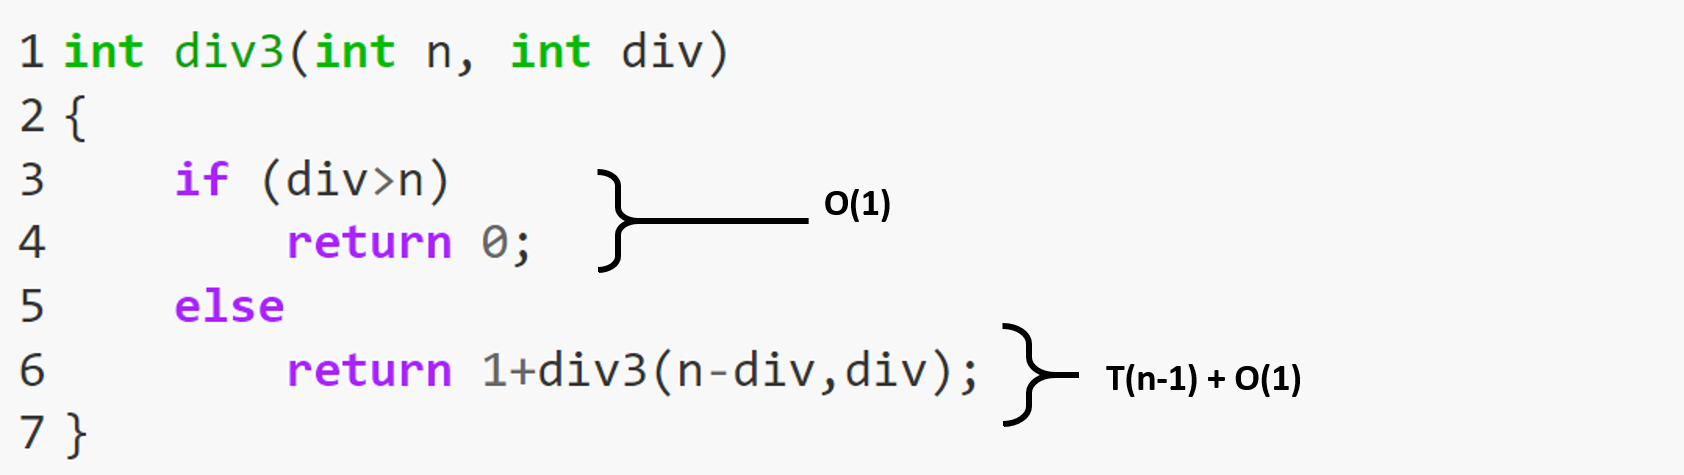
\includegraphics[width=11cm]{imagenes/divc3.png}
                    \caption{Análisis por bloques de código de la función div3().}
                \end{figure}
                
                \newpage
                {\bf 3.1.3.2 Análisis a Posteriori}
                \\[0.3cm]
                
                A continuación se muestra el gráfico de los valores obtenidos. El comportamiento de la gráfica es lineal, sin diferencia entre el     mejor o  el peor caso.
                Se proponen valores para $C_{1}=1$, $C_{2}=3$ y $n_{0}=10$. Dichos valores se acotan la parte superior como la inferior as\'i como el punto de cruce en el que se cumple la desigualdad, por tanto, el algoritmo de la división 3, $T(n)\in O(n)$.


                \begin{figure}[H]
                    \centering
                    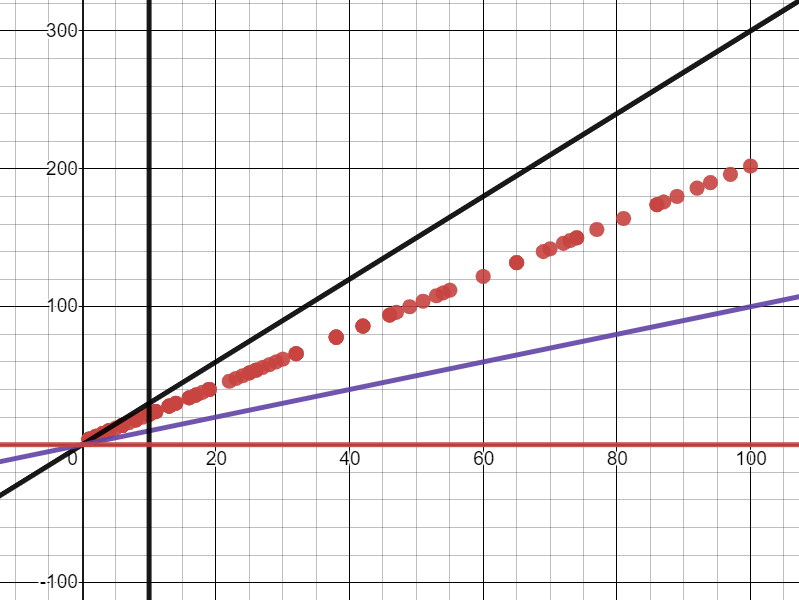
\includegraphics[width=9cm]{imagenes/div3.png}
                    \caption{Gráfico del peor y mejor caso para la función div3().}
                \end{figure}
                
                \begin{figure}[H]
                    \centering
                    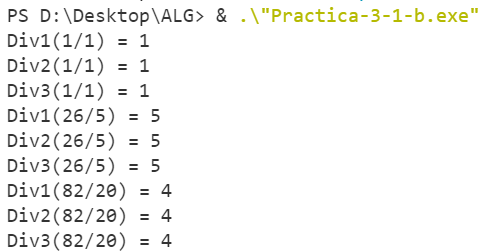
\includegraphics[width=9cm]{imagenes/div_result.png}
                    \caption{Salida del programa al ejecutar div1(), div2() y div3() con los mismas entradas.}
                \end{figure}
                
                Comparando la complejidad de los tres algoritmos anteriores, el algoritmo de división 2 es el más eficiente dado que tiene complejidad logarítmica. Sin embargo, cabe destacar que este algoritmo es el más extenso e implica que posiblemente sea más difícil de comprender por parte del programador, lo que puede llegar a sugerir realizar una buena documentación del algoritmo.
                
        \subsection{B\'usqueda de un elemento en un arreglo en bloques de 3 en 3.}
            El siguiente algoritmo hace la b\'usqueda de un elemento {\it k} en un arreglo de tama\~no {\it n}, bas\'andose en b\'usqueda binaria sin embargo se parte en tres bloque iguales a este, donde dos pivotes {\it i, j} son lo puntos para determinara si el n\'umero se encuentra dentro por medio de comparaciones en cuanto si es mayor, menor o igual a dichas posiciones. Se realizo dos versiones de este algoritmo una iterativa y otra recursiva, en seguida se muestra su an\'alisis a {\it priori} y a {\it posteriori} de cada uno, para determinan cual de estos dos en mas eficiente.  
            \subsubsection{\large Versi\'on iterativa}
            Para esta versi\'on de b\'usqueda se implementa el algoritmo en el lenguaje de programaci\'on C.\\[0.5cm] 
                {\bf 3.2.1.1 Analisis a Priori}\\[0.2cm]
                Por medio de definiciones formales se obtendr\'a la complejidad del algoritmo dado un an\'alisis por secciones de c\'odigo, determinando el tiempo de soluci\'on del problema planteado.\\
               Sin embargo, surge una pregunta , ¿C\'omo obtener la complejidad del {\bf while}?, esta saldra del peor caso que se logre obtener en la reducci\'on del arreglo, siendo que un par\'ametro importante es la condici\'on de la l\'inea 3 de c\'odigo donde se busca que se cumpla que {$inicio\leq final$}, por lo que para el peor caso el tama\~no del arreglo A[] es de 1, así mismo la reducci\'on de este se presenta en la Tabla 1.
               \begin{longtable}{||c|c||}
                    \caption{Complejidad temporal del algoritmo iterativo}\\
                        \hline
                            \textbf{Iteraci\'on}&\textbf{Peor caso T(n)}\\
                         \hline
                            {0}&{$n$}\\
                        \hline
                            {1}&{$\frac{n}{3}$}\\
                        \hline
                            {2}&{$\frac{n}{9}$}\\
                        \hline
                            {3}&{$\frac{n}{27}$}\\
                        \hline
                            {4}&{$\frac{n}{81}$}\\
                        \hline
                            {$\vdots$}&{$\vdots$}\\
                        \hline
                            {k}&{$\frac{n}{3^{K}}$}\\
                        \hline
                \end{longtable}
                Conociendo que el tama\~no del arreglo para el pero caso es 1 y dada la generalizaci\'on del peor caso para las iteraciones del while el orden del complejidad se obtiene de la siguiente igualdad.
                $$\frac{n}{3^{K}}=1$$
                $$entonces,~n=3^{K}$$
                $$luego,~log_3{(n)}=log_3{(3^{K})}$$
                $$\therefore~log_3{(n)}=K$$
                \\
                Dado cada bloque de sentencia del algoritmo, se muestra la obtenci\'on del orden de complejidad para el peor caso de este por medio de un an\'alisis de segmentos de c\'odigo , v\'ease Figura 8, donde se muestra que T(n)$\in O(log_3{(n)})$.
                \begin{figure}[H]
                    \centering
                    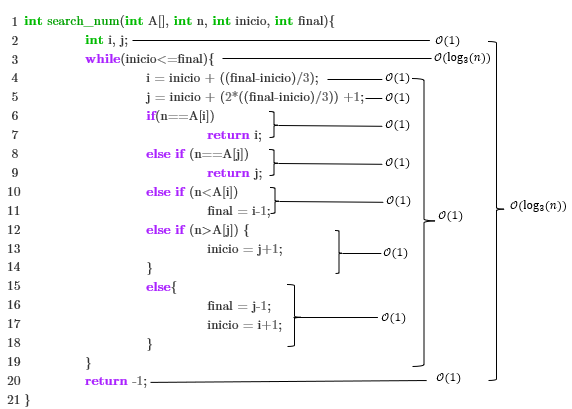
\includegraphics[width=14cm]{imagenes/figura3_2_1.png}
                    \caption{An\'alisis del por bloque de c\'odigo del algoritmo iterativo}
                    \label{fig:my_label}
                \end{figure}
                {\bf 3.2.1.2 Analisis a Posteriori}\\[0.2cm]
                Al ejecutar la funci\'on con el nombre \textit{"search$\_$num"}, se tiene que la asignaci\'on de valores de entrada esta dada por un arreglo A[] y tres enteros que definen el inicio, el final y el n\'umero $n$ a buscar dentro de A[], por tanto al finalizar la ejecuci\'on se obtiene el n\'umero de operaciones que se realizan ante la b\'usqueda de $n$. Posterior a estos se logra obtener los tiempos de ejecuci\'on de tales b\'usquedas, los cuales se muestran en la Figura 9.
                \begin{figure}[H]
                    \centering
                    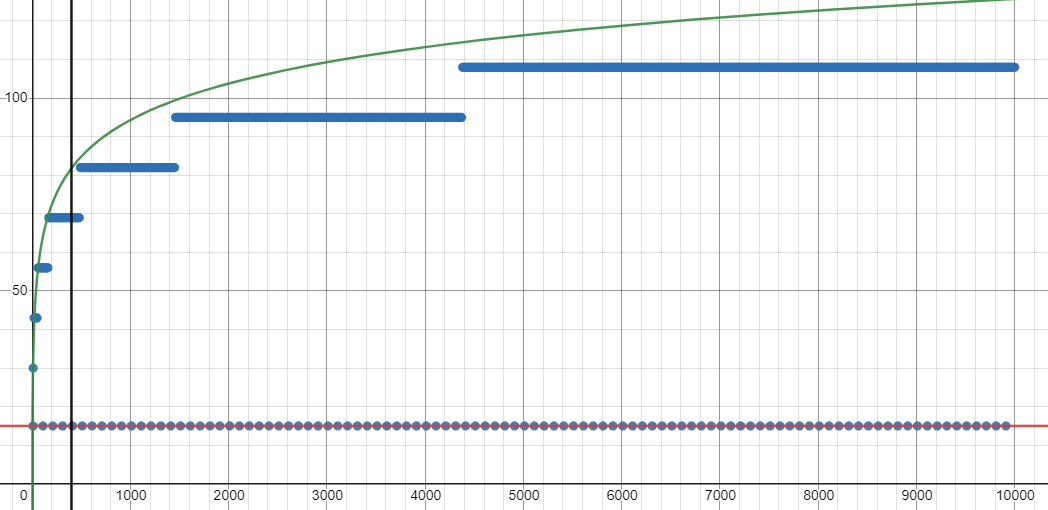
\includegraphics[width=14cm]{imagenes/figura3_2_2.png}
                    \caption{Gráfico del peor y mejor caso para la versi\'on iterativa del algoritmo.}
                \end{figure}
                Ante el resultado de los puntos prueba se determina que el mejor caso es continuo por lo que se puede afirmar que $T(n)~\in~\Omega(1)$, sin embargo para el peor caso se muestra que el crecimiento de los puntos de prueba tiene un comportamiento logar\'itmico por lo que recordando la definici\'on de $\mathcal{O}$:
                $$\mathcal{O}(g(n)) = \{ f(n)~\arrowvert~\exists_{n}~C_{1}>0~\&~n_{1}>0~tal~que$$$$0\leq~f(n)~\leq~C_{1}g(n)~\forall~n\geq~n_{1}\}$$
                Se tiene que $f(n)$ es la funci\'on que acota los resultados no encontrados en A[], sin embargo no se conoce el orden de complejidad de este algoritmo, por lo que proponiendo a $g(n)=log_{3}(n)$, $C_{1}=20$ y $n_{1}=200$ se puede observar que acota por arriba a $f(n)$ por tanto se puede decir que $T(n)~\in~\mathcal{O}(log_{3}(n))$, entonces el algoritmo presenta un orden de complejidad logar\'itmica.
            \subsubsection{\large Versi\'on recursiva}
            La versi\'on recursiva de este algoritmo es implementada en el lenguaje de programaci\'on C.\\[0.5cm]  
                {\bf 3.2.2.1 An\'alisis a Priori}\\[0.2cm]
                La versi\'on recursiva del algoritmo analizado muestra las mismas condiciones para el peor caso de la anterior secci\'on, donde este se presenta cuando el elemento K no se encuentra en un arreglo A[].
                \begin{figure}[H]
                    \centering
                    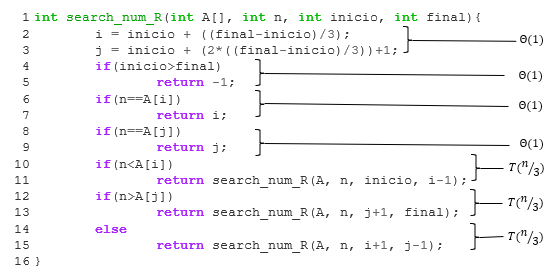
\includegraphics[width=14cm]{imagenes/figura3_2_3.png}
                    \caption{An\'alisis del por bloque de c\'odigo del algoritmo recursivo}
                \end{figure}
                Observando el comportamiento del algoritmo recursivo, divide en 3 partes el arreglo A[], deteni\'endose cuando se cumpla la condici\'on  $inicio>final$ donde la tama\~no del A en este instante es de 1, as\'i mismo cada una de las sentencias condicionales se vuelven constantes por lo que la ecuaci\'on de recurrencia que representa este comportamiento esta dado por:
                $$T(n)= \left\{ \begin{array}{lcc}
                                C &   si  & n=0 \\
                                \\ T(\frac{n}{3})+C &  si & n>0
                                \end{array}
                        \right.$$
                Ahora, sea $n=3^{k}~\Rightarrow~k=\log_3{(n)}$ se tiene que $$T(3^{k})= \left\{ \begin{array}{lcc}
                                C &   si  & k=0\\
                                \\ T(3^{k-1})+C &  si & k>0
                                \end{array}
                        \right.$$\\
                Resolviendo por sustituci\'on hacia atr\'as se tiene\\
                \begin{align}
                    T(3^{k})&=T(3^{k-1})+C\nonumber\\
                    &=(T(3^{k-2})+C)+C=T(3^{k-2})+2C\nonumber\\
                    &=(T(3^{k-3})+C)+2C=T(3^{k-3})+3C\nonumber\\
                    &=(T(3^{k-4})+C)+3C=T(3^{k-4})+4C\nonumber\\
                    &\vdots\nonumber\\
                    &=T(3^{k-i})+iC\nonumber\\
                    para~K=i \Rightarrow K-i=0\nonumber\\
                    &=T(3^{0})+kC\nonumber\\
                    &=T(1)+kC\nonumber\\
                    &=C+kC\nonumber\\
                    &=C+\log_3{(n)}C\nonumber\\
                    \therefore T(n)\in \mathcal{O}(\log_3{(n)})\nonumber
                \end{align}
                
                {\bf 3.2.2.2 An\'alisis a Posteriori}\\[0.2cm]
                Cuando se se hace uso de la funci\'on \textit{$"search\_num\_R"$}, al igual que en su versi\'on iterativa, se obtiene los tiempos de ejecuci\'on $T(n)$ ante la b\'usqueda de un n\'umero $n$ en el arreglo A[]. Al ser graficados estos puntos, muestran el comportamiento que se visualiza en la Figura 11.
                \begin{figure}[H]
                    \centering
                     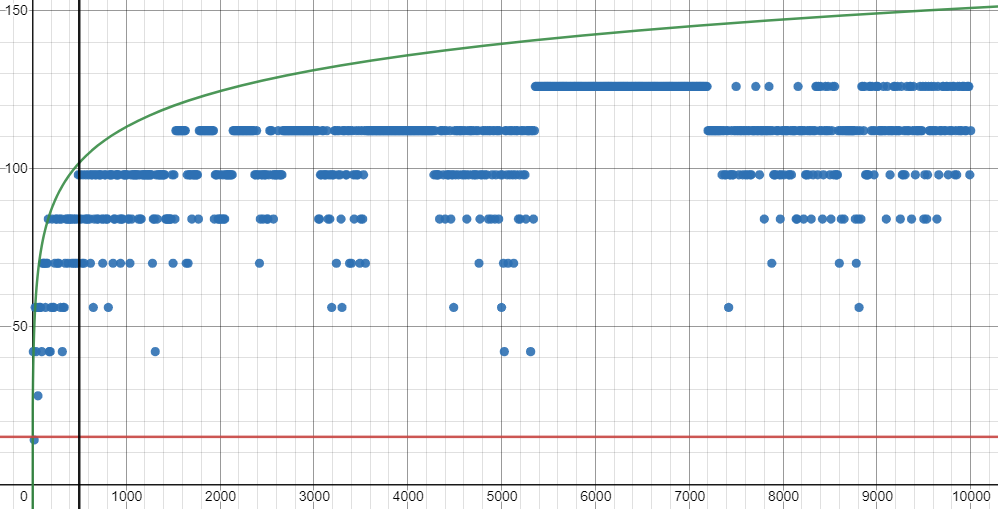
\includegraphics[width=14cm]{imagenes/figura3_2_4.png}
                    \caption{Gráfico del peor y mejor caso para la versi\'on recursiva del algoritmo.}
                \end{figure}
                Al analizar el patr\'on de crecimiento ante el tama\~no del problema se muestra que para el mejor caso el orden de complejidad del algoritmo es constante, as\'i que $T(n)~\in~\Omega(1)$. Por lo que al identificar los puntos prueba que pertenecen a $f(n)$ y que no lograron ser encontrados en A[] muestran un comportamiento logar\'itmico, entonces dada la definici\'on de $\mathcal{O}$:
                $$\mathcal{O}(g(n)) = \{ f(n)~\arrowvert~\exists_{n}~C_{1}>0~\&~n_{1}>0~tal~que$$$$0\leq~f(n)~\leq~C_{1}g(n)~\forall~n\geq~n_{1}\}$$
                Se propone $g(n)=log_{3}(n)$, $C_{1}=16$ y $n_{1}=500$ lo cual es una cota superior para $f(n)$ por lo que se puede decir que $T(n)\in\mathcal{O}(log_{3}(n))$, entonces el algoritmo presenta un orden de complejidad logar\'itmica. 
    \section{Conclusiones}
    \textbf{\large Luis Francisco Renteria Cedillo}
    \begin{figure}[H]
        \centering
        
\includegraphics[angle=0, scale=0.5]{imagenes/foto1.png}
    \end{figure}
    
    Al desarrollar esta práctica, se logró obtener la complejidad computacional de varios algoritmos equivalentes. Un dato importante a mencionar es que las funciones recursivas son más fáciles de comprender que algunas funciones iterativas equivalentes, en especial cuando los algoritmos son cortos, ya que se tienen contempladas las acciones a realizar en cada caso y sabemos que finaliza al llamar la instrucción return junto con una constante. En el caso de que la instrucción return llame a la misma función, es fácil de comprender los argumentos implicados en ella dado que tienen una variación definida que obedece a la definición recurrente de la función
    \newpage
    \textbf{\large Denzel Omar Vazquez Perez}
        \begin{figure}[H]
            \centering
            
\includegraphics[angle=-90, scale= 0.05]{imagenes/foto2.jpg}
        \end{figure}
    La forma en la que se soluciona y codifica problemas, son aspectos que influyen en la determinaci\'on del orden de complejidad que tomara dicho algoritmo, cada uno de los problemas en la practica se tenia visto que se analizar\'ia algoritmos iterativos y recursivos del mismo orden sin embargo, el segundo algoritmo $"Division2"$ mostr\'o tener un orden de cota inferior al de los otros dos por lo se tiene una comparativa una mejor alternativa a los que es la soluci\'on iterativa y recursiva tradicional. Para el segundo problema una de la peculiaridades que se tuvo, sea la soluci\'on iterativa o recursiva tendr\'an ambas la misma complejidad por lo que cualquiera que se emplee sera indistinto para resolver el problema de la b\'usqueda del numero $K$ en el arrglo A[]. 
    \section{Bibliograf\'ia}
    Brassard, G. (1997). \textit {Fundamentos de Algoritmia}. España: Ed. Prentice Hall.\\[0.4cm]
    Cormen, E. A. (2022). \textit{Introduction To Algorithms}, 3Rd Ed. Phi.\\[0.4cm]
    Luna, Benjam\'in. \textit{Fundamentos para el an\'alisis de eficiencia algor\'itmica}. Escuela Superior de Computo, IPN. M\'exico. 03 de abril de 2022.\\[0.4cm]
    S\'anchez, P. J. I. (2006). \textit{Análisis y diseño de algoritmos: un enfoque teórico y práctico}. Servicio de Publicaciones y Divulgación Científica de la UMA.
\end{document}